\begin{chapter}{\label{cha:numerics}Numerical Methods}
\section{\label{section:RK} Numerical procedures for 2D and 3D solutions}
	\subsection{\label{section:RK4} Fourth order Runge-Kutta scheme}
	The classical fourth-order Runge-Kutta formula (RK4) is described equivalently in many texts. We follow the description in \cite{NumericalRecipes}. Let an initial value problem be specified as
	
	\begin{align*}
		\frac{\partial \psi}{\partial t} &= f(\psi,t),\hspace{0.25in}\psi(t_0) = \psi_0.
	\end{align*}

A step-size, $h>0$, is chosen as the parameter controlling how the solution is advanced over $t$. The scheme for estimating $\psi(t_n)= \psi_n$ is then written
\begin{equation}
\begin{split}
		k_1 &= hf(t_n,\psi_n),\\
		k_2 &= hf(t_n+\frac{h}{2},\psi_n+\frac{k_1}{2}),\\
		k_3 &= hf(t_n+\frac{h}{2},\psi_n+\frac{k_2}{2}),\\
		k_4 &= hf(t_n+h,\psi_n+k_3),\\
		\psi_{n+1} &= \psi_n + \frac{k_1}{6}+ \frac{k_2}{3}+ \frac{k_3}{3} + \frac{k_4}{6} + O(h^5),\\
		t_{n+1}  &= t_n + h.
		\label{eq:rk4}
\end{split}
\end{equation}


	A full derivation and proof of accuracy for the RK4 scheme is outlined in Appendix \ref{appsection:rk4deriv}.
	\begin{algorithm}[H]
		\SetKwInOut{Input}{input}\SetKwInOut{Output}{output}
		\Input{An initial field $\Psi$, a step size $h$, optional phase profile $\Theta$}
		\SetKw{KwIn}{in}
		\SetKw{KwAll}{all}
		\SetKw{KwAllPoints}{all points}
		\BlankLine
		$t = 0$\;
		$dt = -ih$\;
		\Repeat{a suitable ground state is found}{
			Perform a single step of the RK4 Scheme\;
			$t = t + dt$\;
			$n\leftarrow \mathrm{norm}(\Psi)$\;
			\For{$\KwAllPoints~i~\KwIn~\Psi$}{
				$\Psi[i]\leftarrow \Psi[i]/\sqrt{n}$\;
			}
			\If{we want a phase profile imprinted into the ground state}{
				\For{$\KwAllPoints~i~\KwIn~\Psi$}{
					$\Psi[i]\leftarrow \Theta[i].|\Psi[i]|$\;
				}
			}
		}
		$dt = h$\;
		\Repeat{satisfied}{
			Perform a single step of the RK4 Scheme\;
			$t = t + dt$\;

			\If{real time normalization is enabled}{
			$n\leftarrow \mathrm{norm}(\Psi)$\;
			\For{$\KwAllPoints~i~\KwIn~\Psi$}{
				$\Psi[i]\leftarrow \Psi[i]/\sqrt{n}$\;
			}
			

			}
		}
	\caption{RK4 algorithm for advancing a ODE/PDE in time. Should normalization of the be required it is included an optional part of this algorithm.}\label{algo_rk4}
	\end{algorithm}

	In all of our relevant calculations the value of f is set as the right hand side of the homogeneous or trapped GPE. The main loop formulating the RK4 method may be repeated indefinitely to reach any $t>t_0$. The step size for a given set of parameters should be chosen small enough that smaller choices make no quantitative changes to the resulting solution.

	\subsection{\label{section:imagTime} The imaginary time propagation method}
	Many numerical explorations of quantum systems, particularly those associated with magnetic or optical trapping,  involve calculating the ground-state as either the final result or as a stepping stone for further calculations. While in theory an expression for the ground-state can be found by considering the lowest-lying eigenvalue (along with its eigenfunction) of the appropriate Hamiltonian, complications arise in calculating the ground-state in the case of the GPE; the non-linearity of the system forces the true ground-state to form as a solution of many simultaneous linear eigenvalue problems.	This complex problem is therefore often solved numerically using so called eigensolvers.

	There are several methods available for implementing a numerical eigensolver: inverse iteration and Lanczos methods \cite{thijssen1999computational}, systematic variational techniques \cite{Bao2003230}, boundary eigenvalue methods \cite{Edwards95}, conjugate gradient techniques \cite{NumericalRecipes} and imaginary time propagation \cite{PhysRevE.62.7438}. We choose to use the last of these methods due to its relative simplicity at the expense of computational time.

	The imaginary time method revolves around moving from real to imaginary time using a Wick rotation $\tau = it$. The substitution transforms the GPE into a form similar to a diffusion equation. As a result, a local equilibrium can be found by propagating $\tau$. This can be understood by considering a trial solution (as similar to the true ground-state as possible) as a collection of eigenfunctions $\Psi_n$ corresponding to eigenvalues $E_n$,
\begin{equation*}
\Psi(\mathbf{r},\tau) = \sum_n \Psi_n(\mathbf{r})\exp\left(-\frac{E_n\tau}{\hbar}\right).
\end{equation*}
The eigenfunctions decay exponentially under propagation of the GPE in imaginary time. In particular, the decay rate is directly related to the size of the eigenvalues $E_n$, so that eigenfunctions relating to higher eigenvalues decay the fastest. The final ingredient is to inhibit the overall decay of the wavefunction by renormalising during propagation. After a sufficient transient time the contributions from the higher eigenvalues become negligible, forcing the wavefunction to tend towards the lowest energy eigenfunction,
\begin{equation*}
\Psi(\mathbf{r},\tau) \rightarrow \Psi_0(\mathbf{r})\exp\left(-\frac{E_0\tau}{\hbar}\right).
\end{equation*}
\begin{figure}
	\centering
	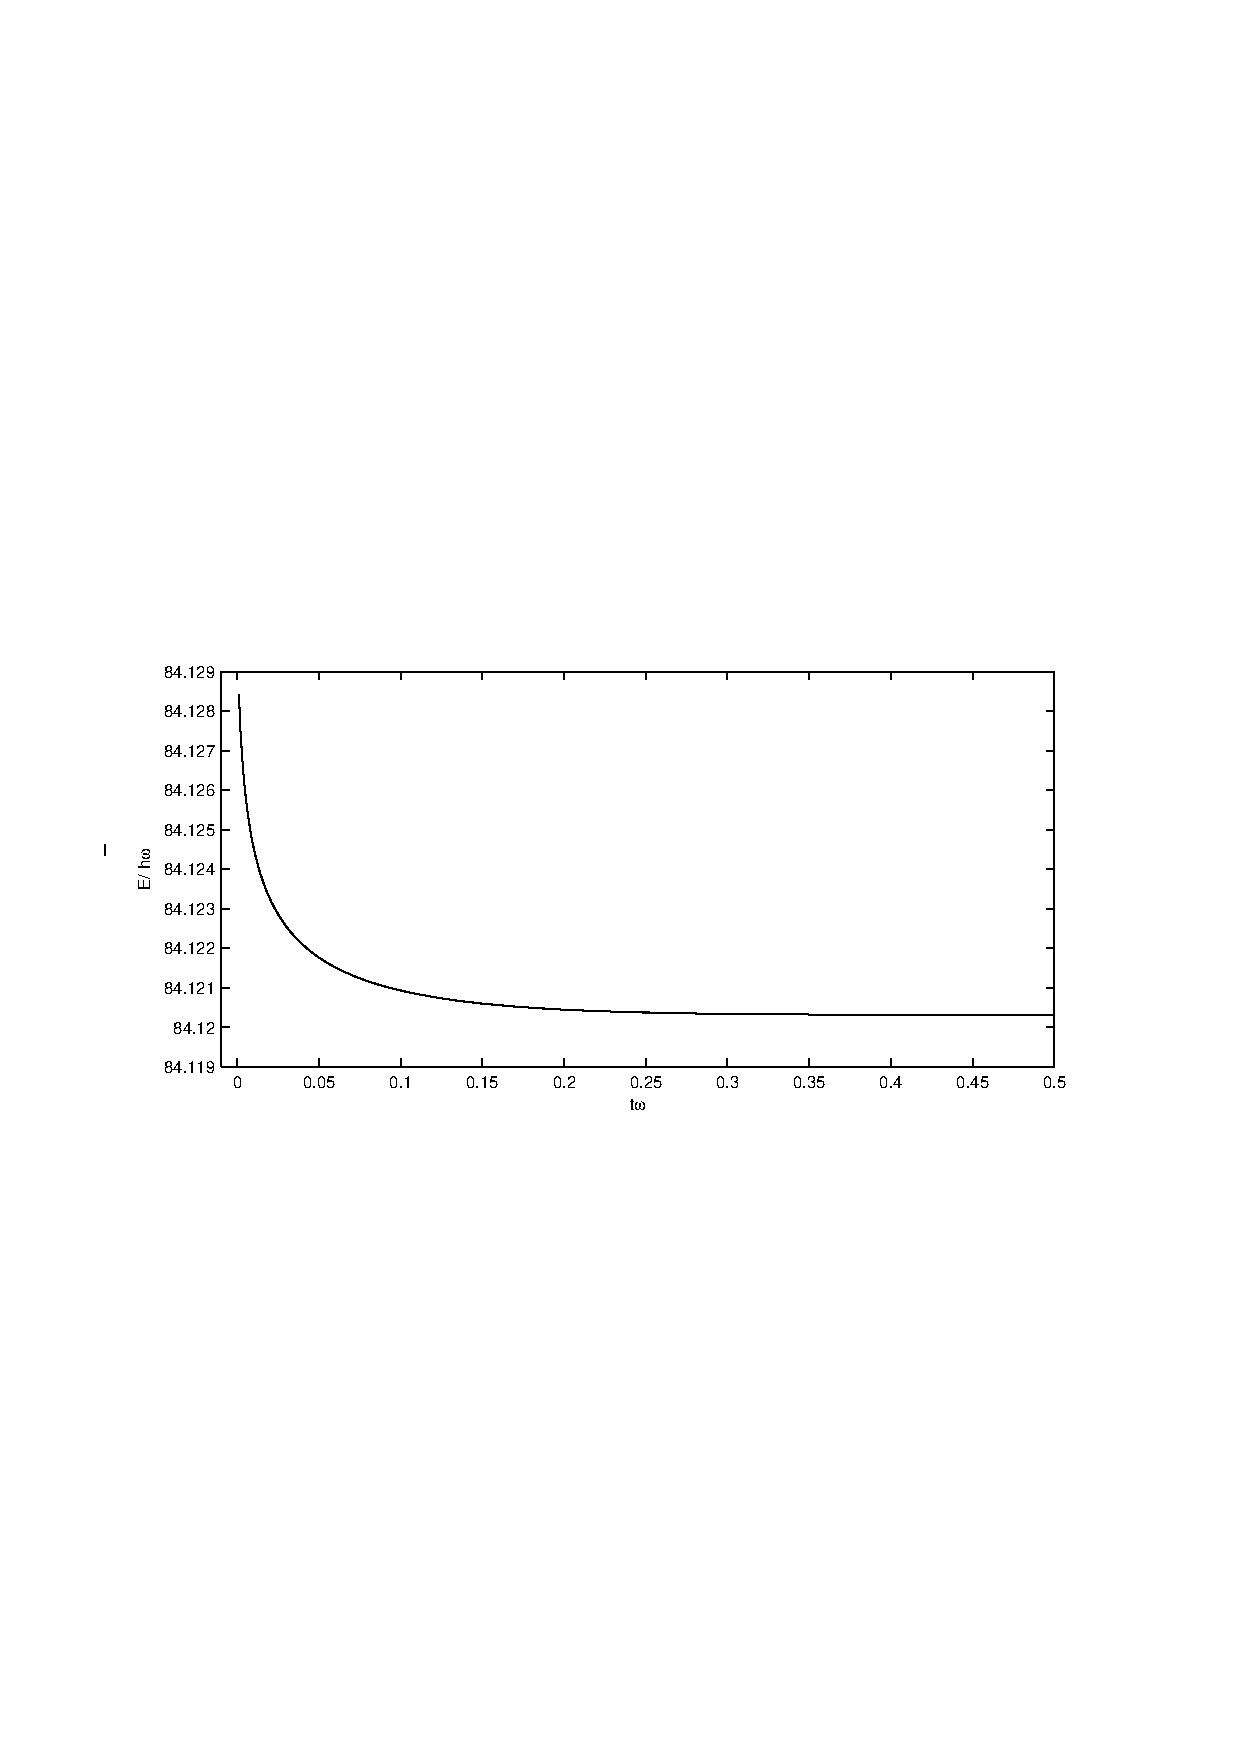
\includegraphics{numerics/figures/imag-time-prop-energy.pdf}
	\includegraphics{numerics/figures/imag-time-gs.pdf}
	\caption{An example of the use of the imaginary time propagation method for finding the condensate ground state for a condensate with interaction energy $\hat{g}=500$ and $\hat{\mu}=12.68$, with the Thomas-Fermi solution as the initial state. The density of the final ground state solution is shown (right) along with the energy of the solution as the method propagates through imaginary time (left).}
\end{figure}
The imaginary time propagation method converges on the ground state solution very slowly and so we must perform many steps to prepare an initial state. A silver lining of this drawback is that the method can be used to prepare almost any viable initial steady state. For example, an initial condition consisting of a Thomas-Fermi profile with many vortices can be `smoothed' by fixing the phase during imaginary time propagation. The result is a less violent start to condensate dynamics as minimal sound is produced due to the difference between the approximate initial condition and a true solution of the GPE.

	\subsection{\label{section:numericalParams} Numerical stability}
	We now systematically study the numerical stability of common simulated systems. Our aim is to find a suitable discretisaton of space and time so that while simulations are timely, our numerical solutions are converged and not overly sensitive to small changes computational parameters.

	We use energy to measure because in the undamped gpe energy is conserved.

	We run 100 units of imaginary time stepping to get density profile
	We run another 100 units for vortex IC
	We run 500 units in real time to study stability


\begin{figure}
	\centering
	\includegraphics[width=0.5\textwidth]{numerics/figures/homg_energy_cons.png}
\end{figure}

\section{\label{section:vortexidentifying} Identifying vortices}

	\begin{algorithm}[H]
	\SetKwFunction{Zero}{Zero}
	\SetKwInOut{Input}{input}\SetKwInOut{Output}{output}
	\Input{A $n_x \times n_y$ wavefunction $\theta$. A $n_x \times n_y$ potential field $V$. A line integral width $l$.}
	\Output{A `vortex field' $Q$.}
	\BlankLine
	\For{$i\leftarrow 1+l/2$ \KwTo $n_x-l/2$}{
		\For{$i\leftarrow 1+l/2$ \KwTo $n_y-l/2$}{
			$Q[i,j]\leftarrow\oint_\Box \nabla\theta~ds$, where $\Box$ is a square loop of width $l$ centered on $(i,j)$\;
		}
		\lIf {$V[i,j]>1$}{$Q[i,j]\leftarrow0$}
	}


\caption{Initial vortex detection. Outputs a field with positive values near a vortex with circulation 1, negative values near a vortex with circulation -1 and zero valued otherwise.}\label{algo_calcvortexfield}
\end{algorithm}
\subsection{\label{section:gaussianblur} Image filters and the Gaussian kernel}
		\begin{algorithm}[H]
		\SetKwInOut{Input}{input}\SetKwInOut{Output}{output}
		\SetKw{KwIn}{in}
		\SetKw{KwAll}{all}
		\SetKw{KwAllPoints}{all points}
		\Input{A $n_x \times n_y$ field $Q$, a Gaussian filter width $g$.}
		\Output{A $n_x \times n_y$ field $G$.}
		\BlankLine
		\For{$\KwAllPoints~i~\KwIn~G$}{
		$G[i]\leftarrow0$\;
		}
		\For{$k\leftarrow 1$ \KwTo $n_x$}{
			\For{$l\leftarrow 1$ \KwTo $n_y$}{
				\For{$i\leftarrow 1$ \KwTo $n_x$}{
					\For{$j\leftarrow 1$ \KwTo $n_y$}{
						$G[k,l] \leftarrow G[k,l] + Q[i,j]\times\exp\left (-[(k-i)^2+(l-j)^2]/g^2 \right )$\;
					}
				}
				$G[k,l] \leftarrow G[k,l]/(n_x.n_y)$\;
			}
		}

	\caption{Gaussian convolution. Filters out features with structures of size less than the input
	filter width. The output is analagous to a `blurring' of the input field. This allows high frequency noise to be removed.}\label{algo_gaussconv}
	\end{algorithm}



	\begin{algorithm}[H]
	\SetKwFunction{Zero}{Zero}
	\SetKwInOut{Input}{input}\SetKwInOut{Output}{output}
	\SetKwData{Mtmp}{m}
	\SetKwFunction{Max}{max}
	\SetKwFunction{Min}{min}
	\SetKw{continue}{continue}
	\SetKw{KwAnd}{and}
	\SetKw{KwIn}{in}
	\SetKw{KwAll}{all}
	\SetKw{KwAllPoints}{all points}
	\Input{A $n_x \times n_y$ binary field $P$.}
	\Output{A $n_x \times n_y$ field $Q$.}
	\BlankLine
	Let $L$ be a $4 \times (n_x.n_y)$ field\;
	Let $A$ be a vector length $4$\;
	\lFor{$\KwAllPoints~i~\KwIn~L$}{
	$L[i]\leftarrow-1$
	}
	\lFor{$\KwAllPoints~i~\KwIn~Q$}{
	$Q[i]\leftarrow-1$
	}

	$l_c\leftarrow 1$, $r_c\leftarrow 0$\;

	\For{$i\leftarrow 2$ \KwTo $n_x-1$}{
		\For{$j\leftarrow 2$ \KwTo $n_y-1$}{
			\lIf {$P[i,j] = 0$}{\continue}
			$A \leftarrow (Q[i+1,j-1],Q[i,j-1],Q[i-1,j-1],Q[i-1,j])$\;
			\For{$c \leftarrow 1$ \KwTo $4$}{
				\If {$A[c]\geq 0$}{
					$Q[i,j]\leftarrow A[c]$\;
					$L[c,l_c]\leftarrow A[c]$\;
				}
			}
			\lIf{$Q[i,j] \geq 0$}{$l_c\leftarrow lc+ 1$}
			\Else{
				$Q[i,j]\leftarrow r_c $\;
				$rc \leftarrow r_c+ 1$\;
			}
		}
	}
	\For{$r\leftarrow 1$ \KwTo $(n_x.n_y)$}{
		\lIf{\Max{elements of $L$ in row $r$}$= -1$}{\continue}
		$m\leftarrow$ \Min{elements of $L$ in row $r$ with value $\geq 0$}\;

		\For{$c\leftarrow 1$ \KwTo $4$}{
			\If{$L[c,r] \neq m$ \KwAnd $L[c,r] \geq 0$ }{
				\For{$\KwAllPoints~i~\KwIn~Q$}{
					\lIf{$Q[i]=L[c,r]$}{$Q[i] \leftarrow m$}
				}
			}
		}
	}


\caption{The B/W Label algorithm. Outputs a field with the same non-zero regions of the input binary field, but with each connected region labeled with a unique value.}\label{algo_bwlabel}
\end{algorithm}


	\begin{algorithm}[H]
	\SetKwFunction{Zero}{Zero}
	\SetKwInOut{Input}{input}\SetKwInOut{Output}{output}
	\SetKwData{Linked}{linked}
	\SetKw{KwAnd}{and}
	\SetKwFunction{Max}{max}
	\SetKwFunction{Min}{min}
	\SetKwData{Call}{C}
	\Input{A $n_x \times n_y$ field $\theta$. A $n_x \times n_y$ field $P$. A threshold value $t$.}
	\Output{Number of vortices found, $n_v$. Vortex location, a $2 \times n_v $ field $V_l$. Vortex polarity, a vector $V_p$ of length $n_v$.}
	\BlankLine
	$Q\leftarrow$ Algorithm \ref{algo_gaussconv} $\leftarrow$ Algorithm \ref{algo_calcvortexfield} $\leftarrow(\theta,P)$ \;
	$R\leftarrow0$ at every point, $S\leftarrow0$ at every point\;
	$n_v\leftarrow 0$\;
	\For{$i\leftarrow 1$ \KwTo $n_x$}{
		\For{$j\leftarrow 1$ \KwTo $n_y$}{
			\lIf {$Q[i,j]>t$}{$R[i,j] = 1$}
			\lIf {$Q[i,j]<t$}{$S[i,j] = 1$}
		}
	}

	\ForEach{$C\in(R,S)$}{
		$D\leftarrow$ Algorithm \ref{algo_bwlabel} $\leftarrow C$\;
		\For{$i\leftarrow 1$ \KwTo \Max($D$)}{
			$V[1,n_v]\leftarrow$ mean row of the points where $D=i$\;
			$V[2,n_v]\leftarrow$ mean column of the points where $D=i$\;
			\lIf {$C=R$}{$V[3,n_v]\leftarrow 1$}
			\lIf {$C=S$}{$V[3,n_v]\leftarrow -1$}
			$n_v \leftarrow n_v + 1$\;
		}
	}

	\caption{Calculate vortex locations and polarity.}\label{algo_calcvortexlocs}
	\end{algorithm}



\section{\label{section:vortexclustering} Quantifying vortex clustering}
	\subsection{\label{section:reevesalgorithm} Recursive Cluster Algorithm (RCA) }
		\begin{algorithm}[H]
		\SetKwFunction{Zero}{Zero}
		\SetKwInOut{Input}{input}\SetKwInOut{Output}{output}
		\SetKwData{Linked}{linked}
		\SetKw{KwAnd}{and}
		\SetKwFunction{Max}{max}
		\SetKwFunction{Min}{min}
		\SetKw{continue}{continue}
		\SetKw{or}{or}
		\SetKw{and}{and}
		\SetKwData{Call}{C}
		\Input{Vortex location, a $2 \times n_v $ field $V_l$. Vortex polarity, a vector $V_p$ of length $n_v$. Number of vortices, $n_v$.}
		\Output{Vortex decomposition, a vector $V_{\mathrm{rca}}$ of length $n_v$.}
		\BlankLine
		$n_{\mathrm{rca}}\leftarrow0$\;
		$V_{\mathrm{rca}}\leftarrow 0$ at every point\;
		\While{dipoles continue to be identified}{
			\For{$i\leftarrow 1$ \KwTo $n_v$}{
				\If {vortex $i$ is mutual nearest neighbours with some other vortex $j$}{
				\If {$V_p[i] \neq V_p[i]$}{
						$V_{\mathrm{rca}}[i] \leftarrow -1$\;
						$V_{\mathrm{rca}}[j] \leftarrow -1$\;
					}
				}
			}
		}
		\While{vortices continue to be added to clusters}{
			\For{$i\leftarrow 1$ \KwTo $n_v$}{
				\For{$j\leftarrow 1$ \KwTo $n_v$}{
					\lIf {$V_{\mathrm{rca}}[i] < 0$ \or $V_{\mathrm{rca}}[j]<0$}{\continue}
					\If {vortex $i$ and $j$ are closer to one another than one of opposite polarity}{
						\lIf {$V_{\mathrm{rca}}[i] > 0$ \and $V_{\mathrm{rca}}[j] = 0$}{$V_{\mathrm{rca}}[j]\leftarrow V_{\mathrm{rca}}[i]$}
						\lElseIf {$V_{\mathrm{rca}}[i] = 0$ \and $V_{\mathrm{rca}}[j] > 0$}{$V_{\mathrm{rca}}[i]\leftarrow V_{\mathrm{rca}}[j]$}
						\lElseIf {$V_{\mathrm{rca}}[i] > 0$ \and $V_{\mathrm{rca}}[j] > 0$}{(All $V_{\mathrm{rca}}=V_{\mathrm{rca}}[i]) \leftarrow V_{\mathrm{rca}}[j]$}
						\Else{
							$n_{\mathrm{rca}} \leftarrow n_{\mathrm{rca}} + 1$\;
							$V_{\mathrm{rca}}[i]\leftarrow n_{\mathrm{rca}}$\;
							$V_{\mathrm{rca}}[j]\leftarrow n_{\mathrm{rca}}$\;
							}
					}
				}
			}
		}

		\caption{The Recursive Cluster Algorithm. Decomposes a list of vortices into vortex dipoles or clusters. Vortices are labelled with a cluster number, with vortex dipoles labelled with $-1$.}\label{algo_rca
		}
		\end{algorithm}


	\subsection{\label{section:ripleysk} Ripley's K function }
		\begin{equation}\label{eq:ripleysk}
		K(x) = \frac{A}{n^2}\sum\limits_{i \ne j} I\left (d_{ij}<x\right ),
		\end{equation}
		where $d_{ij}$ is the distance between the $i$th and $j$th points, $A$ is the area of the region containing every point, $n$ is the number of points, $x$ is the search radius, and I is the indicator function (1 if its argument is true, 0 otherwise). Should the points be distributed homogeneously in space, then $K(s)\approx\pi s^2$.
\section{\label{section:vortextracking} Tracking vortex trajectories}
\section{\label{section:vortexremoval} Removing vortices with phase unwrapping}
	\begin{algorithm}[H]
	\SetKwFunction{Zero}{Zero}
	\SetKwInOut{Input}{input}\SetKwInOut{Output}{output}
	\SetKwData{Linked}{linked}
	\SetKw{KwAnd}{and}
	\SetKwFunction{Max}{max}
	\SetKwFunction{Min}{min}
	\SetKwFunction{Phase}{phase}
	\SetKwData{Call}{C}
	\Input{A $n_x \times n_y$ complex field $\psi$. A `safe' distance $d$. Vortex core radius $c$. }
	\Output{A $n_x \times n_y$ complex field $\phi$.}
	\BlankLine
	$\phi \leftarrow \psi$\;
	$(n_v,V_l,V_p)\leftarrow$ Algorithm \ref{algo_calcvortexlocs}~$\leftarrow\psi$\;

	\For{$i\leftarrow 1$ \KwTo $n_v$}{
		\If{$|V_l[i]| > d$}{
			Imprint a vortex of polarity $V_p[i]$ at location $V_l[i]$ in $\phi$\;
			\For{$j\leftarrow -c$ \KwTo $c$}{
				\For{$k\leftarrow -c$ \KwTo $c$}{
						$x \leftarrow V_l[1,i]+j$\;
						$y \leftarrow V_l[2,i]+k$\;
						\mbox{$\phi(x,y) \leftarrow \psi_{\inf}~\times$~\Phase{$\psi(x,y)$}\;}
				}
			}
		}
	}

	\caption{The `vortex killer' algorithm. By accurately imprinting a vortex, this algorithm removes vortices from the input wavefunction non destructively.}\label{algo_vortexkiller}
	\end{algorithm}

\end{chapter}
